\section{Problema a trabajar}

El problema a trabajar va a ser el de un sistema clasificador, que recibe datos de distintos tipos y luego devuelve una clase asociada a esos datos. Por ahora las clases asociadas a los datos pueden dos, Positiva y Negativa, siendo un problema de clasificaci\'on binaria. Los datos que recibe el sistema son luego de forma parcial o total observados por distintos modelos clasificadores que dan cada uno su resultado individual. Luego esos resultados son puestos en com\'un por un fusionador, que devuelve una \'unica clase para cada dato asociado.

Los modelos corren en paralelo, y de forma independiente donde cada uno mira parte del dato de entrada y devuelve su resultado, sin depender de otros modelos.

\vspace{6mm}

\begin{center}
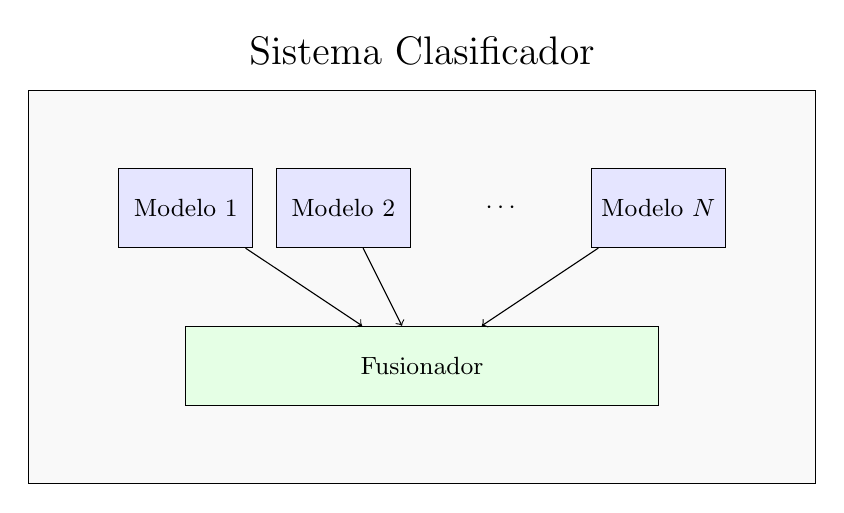
\begin{tikzpicture}[
        every node/.style={font=\small},
        modelo/.style={draw, fill=blue!10, minimum width=1.7cm, minimum height=1cm},
        fusionador/.style={draw, fill=green!10, minimum width=6cm, minimum height=1cm},
        sistema/.style={draw, fill=gray!5}
    ]

    % Sistema
    \node[font=\Large] (titulo) at (0,3) {Sistema Clasificador};
    \node[sistema, minimum width=10cm, minimum height=5cm] (sistema) at (0,0) {};

    % Modelos
    \node[modelo] (modelo1) at (-3,1) {Modelo 1};
    \node[modelo] (modelo2) at (-1,1) {Modelo 2};
    \node at (1,1) {$\cdots$};
    \node[modelo] (modeloN) at (3,1) {Modelo $N$};

    % Fusionador
    \node[fusionador] (fusionador) at (0,-1) {Fusionador};

    % Aristas
    \draw[->] (modelo1) to (fusionador);
    \draw[->] (modelo2) to (fusionador);
    \draw[->] (modeloN) to (fusionador);
\end{tikzpicture}
\end{center}

El objetivo es encontrar alguna funci\'on con la cual evaluar uno de los modelos del sistema, sin la necesidad de correr el sistema completo. Al evaluar el modelo con esa funci\'on, se debe obtener informaci\'on relevante del sistema solo al ejecutarla en el modelo. Esto no significa que para definir la funci\'on no se pueda correr el sistema completo. Por lo tanto el planteo es encontrar una funci\'on que de informaci\'on relevante, construida en base al sistema en el que el modelo se va a ejecutar, pero con un hueco en el lugar del modelo. Esta funci\'on debe tener al modelo como par\'ametro. Luego se utiliza independiente al sistema en cualquier posible modelo que vaya a ocupar ese lugar.

\begin{center}
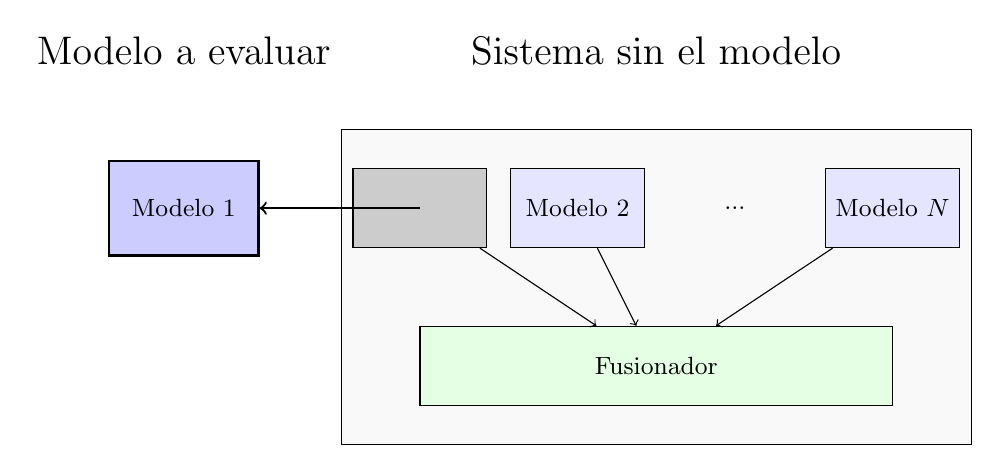
\begin{tikzpicture}[
        every node/.style={font=\small},
        modelo/.style={draw, fill=blue!10, minimum width=1.7cm, minimum height=1cm},
        fusionador/.style={draw, fill=green!10, minimum width=6cm, minimum height=1cm},
        sistema/.style={draw, fill=gray!5}
    ]

    % Modelo externo
    \node[font=\Large] (titulo) at (-6,3) {Modelo a evaluar};
    \node[modelo, fill=blue!20, thick, minimum width=1.9cm, minimum height=1.2cm] (modeloEvaluar) at (-6,1) {Modelo 1};

    % Sistema
    \node[font=\Large] (titulo) at (0,3) {Sistema sin el modelo};
    \node[sistema, minimum width=8cm, minimum height=4cm] (sistema) at (0,0) {};

    % Modelos
    \node[modelo, fill=gray!40] (modelo1) at (-3,1) {};
    \node[modelo] (modelo2) at (-1,1) {Modelo 2};
    \node at (1,1) {...};
    \node[modelo] (modeloN) at (3,1) {Modelo $N$};

    % Fusionador
    \node[fusionador] (fusionador) at (0,-1) {Fusionador};

    % Aristas
    \draw[->] (modelo1) to (fusionador);
    \draw[->] (modelo2) to (fusionador);
    \draw[->] (modeloN) to (fusionador);
    \draw[->, thick] (-3,1) to (modeloEvaluar);
\end{tikzpicture}
\end{center}

Para representar el funcionamiento del sistema en cierta poblaci\'on de datos, voy a usar Redes Bayesianas Causales.


\subsection{Redes bayesianas causales}

Una Red Bayesiana es un Grafo Ac\'iclico Dirigido, donde se representan distribuciones de probabilidad conjuntas. Se separan variables aleatorias en nodos y se vinculan a otras con aristas, representando probabilidades condicionales, asi definiendo la distribuci\'on completa de forma eficiente. Una Red Bayesiana Causal es una Red Bayesiana cuyas aristas agregan un significado de causalidad de nodos padres a nodos hijos sobre el significado probabilistico de las Redes Bayesianas\cite{koller2009probabilistic}. Los nodos con doble c\'irculo representan que son deterministicos dados sus padres.

Para el problema a tratar, voy a modelar con un nodo raiz la poblaci\'on de datos, del cual depende la Clase a la que pertenecen y las distinas features que se observan sobre ese dato. Luego esas features son analizadas por el sistema y por \'ultimo se consigue una predicci\'on y su confusi\'on asociada dependiendo de la clase a la que pertenece ese dato.

\begin{center}
\begin{tikzpicture}[
        scale=1, every node/.style={font=\large},
        fontSize/.style={font=\large}
    ]

    % Descripcion
    \node[draw, fill=blue!30, minimum width=12cm, minimum height=6cm] at (0,7.75) (Sistema) {}; 
    \node[font=\huge, right = 0.1cm of Sistema] (Descripcion Sistema) {\textcolor{blue}{\textbf{Sistema}}};
    
    % Instancias
    \node[latent, fontSize, fill=green!10] at (0,15) (Instancia) {$Instancia$};
    \node[latent, fontSize, double, fill=green!40] at (8,13.5) (Clase) {$Clase$};
    
    % Features
    \node[latent, fontSize, fill=green!10] at (-4.5,12) (Feature1) {$Feature1$};
    \node[latent, fontSize, fill=green!10] at (-1.5,12) (Feature2) {$Feature2$};
    \node[fontSize] at (1.5,12) (FeatureI) {...};
    \node[latent, fontSize, fill=green!10] at (4.5,12) (FeatureN) {$FeatureN$};
    
    % Modelos
    \node[latent, fontSize, fill=blue!20] at (-4.5,9) (Pred M1) {$Pred^{M1}$};
    \node[latent, fontSize, fill=blue!20] at (-1.5,9) (Pred M2) {$Pred^{M2}$};
    \node[fontSize] at (1.5,9) (Pred Mi) {...};
    \node[latent, fontSize, fill=blue!20] at (4.5,9) (Pred Mn) {$Pred^{Mn}$};
    
    % Outputs
    \node at (0,6.5) (Fusionador) {\textbf{fusionador}};
    \node[latent, fontSize, fill=red!20] at (0,3) (Pred S) {$Pred^S$};
    \node[latent, fontSize, double, fill=red!10] at (0,0) (Conf S) {$Conf^S$};

    % Aristas
    \draw[->] (Instancia) to (Clase);

    \draw[->] (Instancia) to (Feature1);
    \draw[->] (Instancia) to (Feature2);
    \draw[->] (Instancia) to (FeatureN);

    \draw[->] (Feature1) to node[right] {\textbf{modelo 1}} (Pred M1);
    \draw[->] (Feature2) to node[right] {\textbf{modelo 2}} (Pred M2);
    \draw[->] (FeatureN) to node[left] {\textbf{modelo n}} (Pred Mn);

    \draw[->] (Pred M1) to (Pred S);
    \draw[->] (Pred M2) to (Pred S);
    \draw[->] (Pred Mn) to (Pred S);

    \draw[->] (Pred S) to (Conf S);
    \draw[->] (Clase.south east) to[bend left] (Conf S.east);
\end{tikzpicture}
\end{center}


\subsection{Ejemplo a analizar}

Empiezo usando un sistema en particular para analizar y intentar generalizar a otros casos. Tengo un sistema con dos modelos en paralelo, cada uno con datos de entrada distintos. Uno por ejemplo podr\'ia recibir im\'agenes m\'edicas y el otro la historia cl\'inica de un paciente, cada uno clasificando el estado del paciente (Positivo o Negativo) de forma independiente. Luego sus resultados son pasados a un fusionador que se encarga de unificarlos y devolver un único resultado para todo el sistema.

\begin{center}
\begin{tikzpicture}[
        scale=1, every node/.style={font=\large},
        fontSize/.style={font=\large}
    ]

    % Descripcion
    \node[draw, fill=blue!30, minimum width=9.5cm, minimum height=6.5cm] at (0,7.75) (Sistema) {};
    \node[font=\huge, right = 0.1cm of Sistema] (Descripcion Sistema) {\color{blue} \textbf{Sistema}};
    
    % Instancias
    \node[latent, fontSize, fill=green!10] at (0,15) (Persona) {$Persona$};
    \node[latent, fontSize, double, fill=green!40] at (5,13) (Clase) {$Clase$};
    
    % Features
    \node[latent, fontSize, fill=green!10] at (-2,12) (Imagen) {$Imagen$};
    \node[latent, fontSize, fill=green!10] at (2,12) (Historia) {$Historia$};
    
    % Modelos
    \node[latent, fontSize, fill=blue!20] at (-2,9) (Pred M1) {$Pred^{M1}$};
    \node[latent, fontSize, fill=blue!20] at (2,9) (Pred M2) {$Pred^{M2}$};
    \node[latent, fontSize, double, fill=blue!10] at (-3,6) (Conf M1) {$Conf^{M1}$};
    \node[latent, fontSize, double, fill=blue!10] at (3,6) (Conf M2) {$Conf^{M2}$};
    
    % Outputs
    \node[latent, fontSize, fill=red!20] at (0,3) (Pred S) {$Pred^S$};
    \node[latent, fontSize, double, fill=red!10] at (0,0) (Conf S) {$Conf^S$};
    \node at (0,6.5) (Fusionador) {\textbf{fusionador}};

    % Aristas
    \draw[->] (Persona) to (Clase);
    \draw[->] (Persona) to (Imagen);
    \draw[->] (Persona) to (Historia);
    \draw[->] (Imagen) to node[left] {\textbf{modelo 1}} (Pred M1);
    \draw[->] (Historia) to node[right] {\textbf{modelo 2}} (Pred M2);
    \draw[->] (Pred M1) to (Conf M1);
    \draw[->] (Pred M2) to (Conf M2);
    \draw[->] (Pred M1) to (Pred S);
    \draw[->] (Pred M2) to (Pred S);
    \draw[->] (Pred S) to (Conf S);
    \draw[->] (Clase) to[bend left] (Conf M1.east);
    \draw[->] (Clase.280) to[bend left] (Conf M2.north east);
    \draw[->] (Clase.south east) to[bend left] (Conf S.east);
\end{tikzpicture}
\end{center}


\subsection{Intervenci\'on}